%! Author = tstreule

\section{Action Potential \& Hodgkin-Huxley Model}
%%%%%%%%%%%%%%%%%%%%%%%%%%%%%%%%%%%%%%%%%%%%%%%%%%%%%%
%%%%%%%%%%%%%%%%%%%%%%%%%%%%%%%%%%%%%%%%%%%%%%%%%%%%%%
\begin{minipage}[t]{.5\columnwidth-.5\columnsep}
    \subsection{Current Clamp}
    %
    \textbf{Fix current} $I_m$ and\\
    measure membrane potential
    \begin{itemize}
        \item[$\to\!\!$] Good for observing AP\\
        (since voltage can change)
    \end{itemize}
\end{minipage}%
\hspace{\columnsep}%
\begin{minipage}[t]{.5\columnwidth-.5\columnsep}
    \subsection{Voltage Clamp}
    %
    \textbf{Fix voltage} $V_m$ and\\
    measure the current
    \begin{itemize}
        \item[$\to\!\!$] Good for studying membrane channel proteins (ion transp.)
    \end{itemize}
\end{minipage}
%%%%%%%%%%%%%%%%%%%%%%%%%%%%%%%%%%%%%%%%%%%%%%%%%%%%%%
\subsection{2-state ion channel model}
%
\formula{two states}{\ce{close <=>[\alpha][\beta] open}}
\quad with gate charge $Q$
\formula{\#open states}{\deriv{n(t)}{t} = \alpha (\mathcal{N} - n(t)) - \beta n(t)}
\formbox{Prob. being open}{x(t) \simeq \frac{n(t)}{\mathcal{N}} = x_\infty\! + (x_0-x_\infty\!) \;\eu^{-t/\tau_x}}
\formbox{~}{x_\infty\! = \frac{\alpha}{\alpha+\beta}, \quad \tau_x = \frac{1}{\alpha+\beta}}

\begin{minipage}{\linewidth}
    \begin{minipage}{\linewidth}
        \formula{Boltzmann law}{\alpha = A\;\eu^{(E_c-E_B)/kT}}
        \formula{~}{\beta = A\;\eu^{(E_o-E_B)/kT}}
        \formula{~}{x_\infty\! = \frac{1}{1+\beta/\alpha} = \frac{1}{1+\eu^{-QV_m/kT}}}
        \formula{~}{\tau_x = \frac{1}{A\;\eu^{-\frac{1}{2}QV_B/kT}} \cdots}
        \formula{~}{\phantom{\tau_x =} \cdots \frac{1}{\eu^{\frac{1}{2}QV_m/kT} + \eu^{-\frac{1}{2}QV_m/kT}}}
    \end{minipage}
    \begin{minipage}{\linewidth}
        \vspace{-30mm}\hfill
        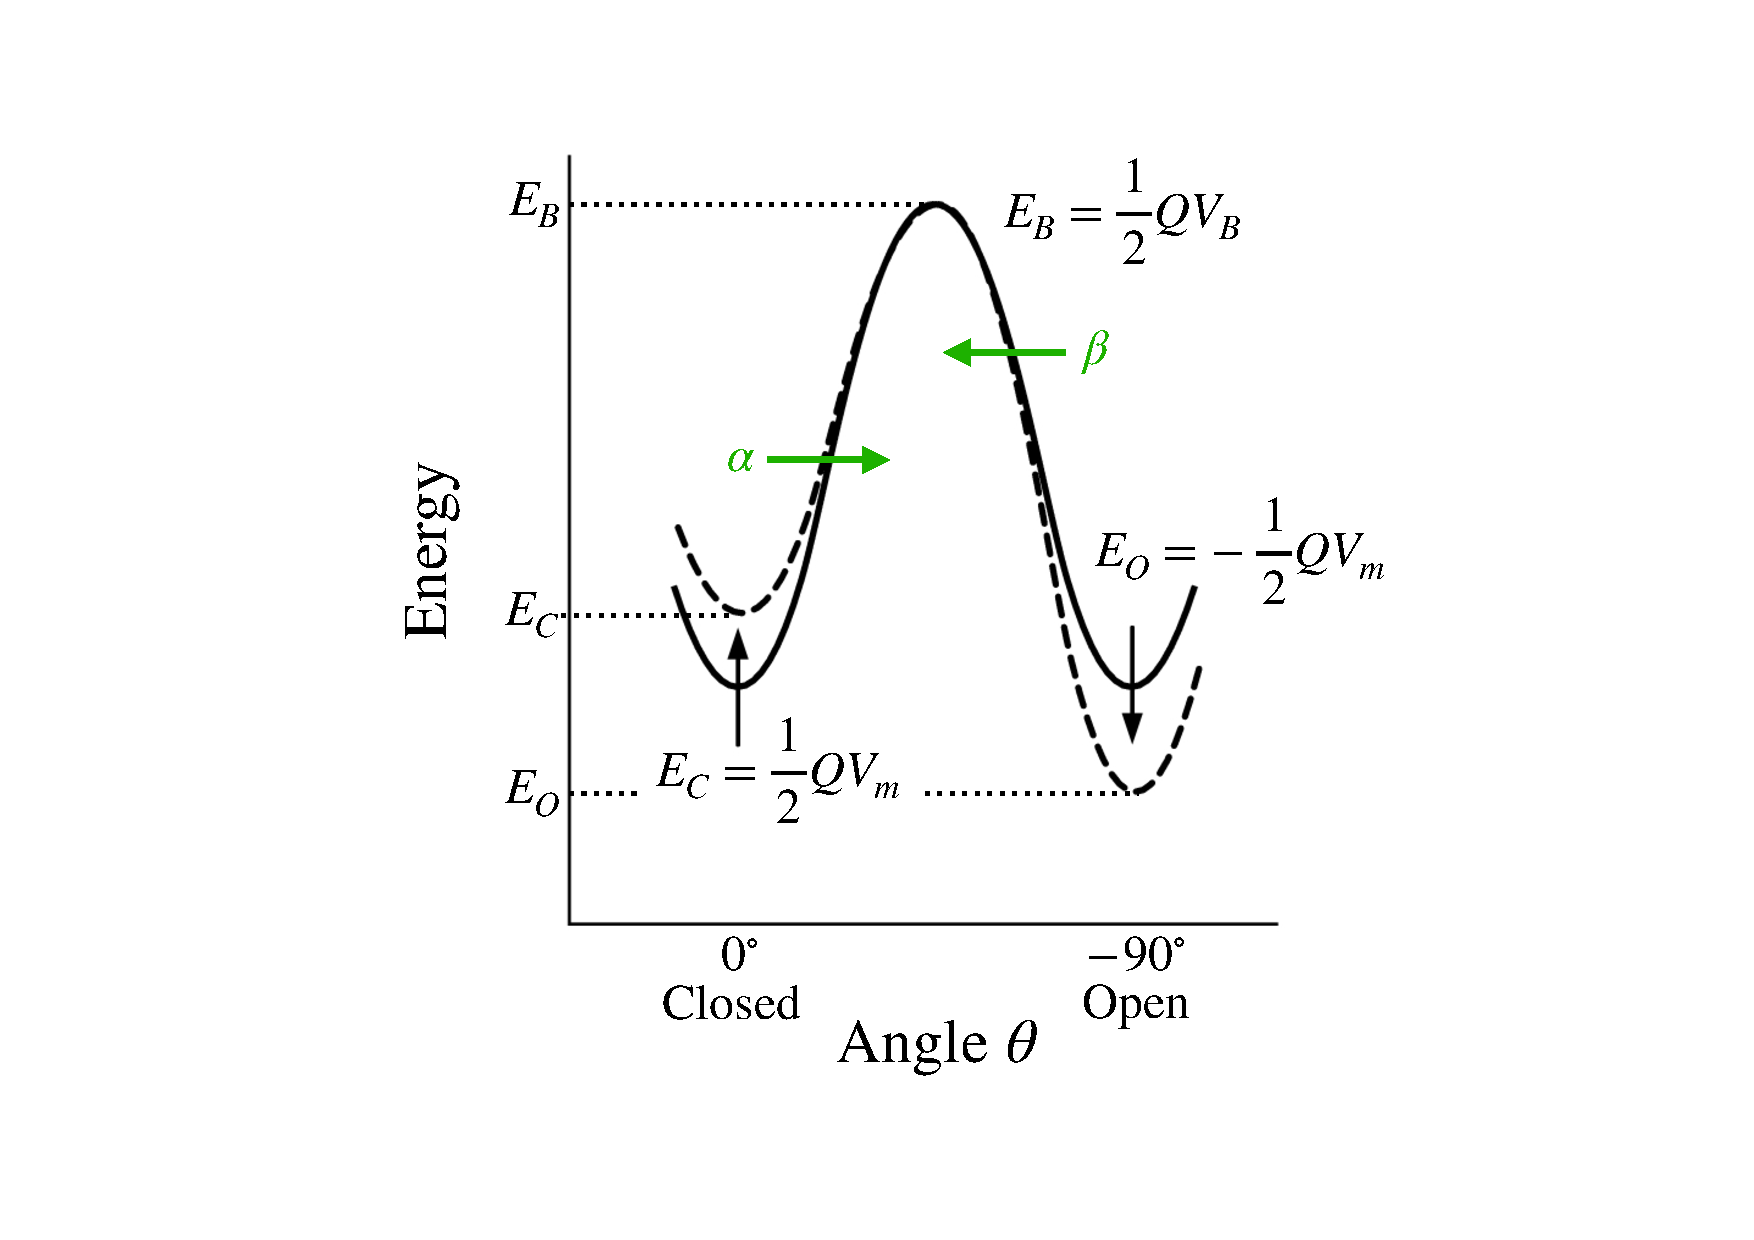
\includegraphics[width=.35\columnwidth]{AP_Boltzmann}
    \end{minipage}
\end{minipage}
%%%%%%%%%%%%%%%%%%%%%%%%%%%%%%%%%%%%%%%%%%%%%%%%%%%%%%
\subsection{Circuit Model \textnormal{(Conductance) \hfill\small$V\ped{K} \simeq \unit[-75]{mV}, \quad V\ped{Na} \simeq \unit[+55]{mV}$}}
%
\formtex{~}{\scalebox{.9}{%
    \highlight{$J\ped{C} = C_m \deriv{V_m(t)}{t}$} \enskip \fbox{$J_m = C_m \deriv{V_m}{t} + G_m(V_m-V_m\ap{rest})$}}}
\formtex{~}{\scalebox{.9}{%
    \highlight{$J\ped{K} = G\ped{K}\;(V_m-V\ped{K})$} \scriptsize always $>0$, we don't fall below ($V_m>V\ped{K}$)}}
\formtex{~}{\scalebox{.9}{%
    \highlight{$J\ped{Na} = G\ped{Na}\;(V_m-V\ped{Na})$} \scriptsize $\begin{cases}>0 & \text{if } V_m-V\ped{Na}>0 \\ <0 & \text{otw.} \end{cases}$}}

\vspace{-18mm}%
\begin{minipage}{\linewidth}
    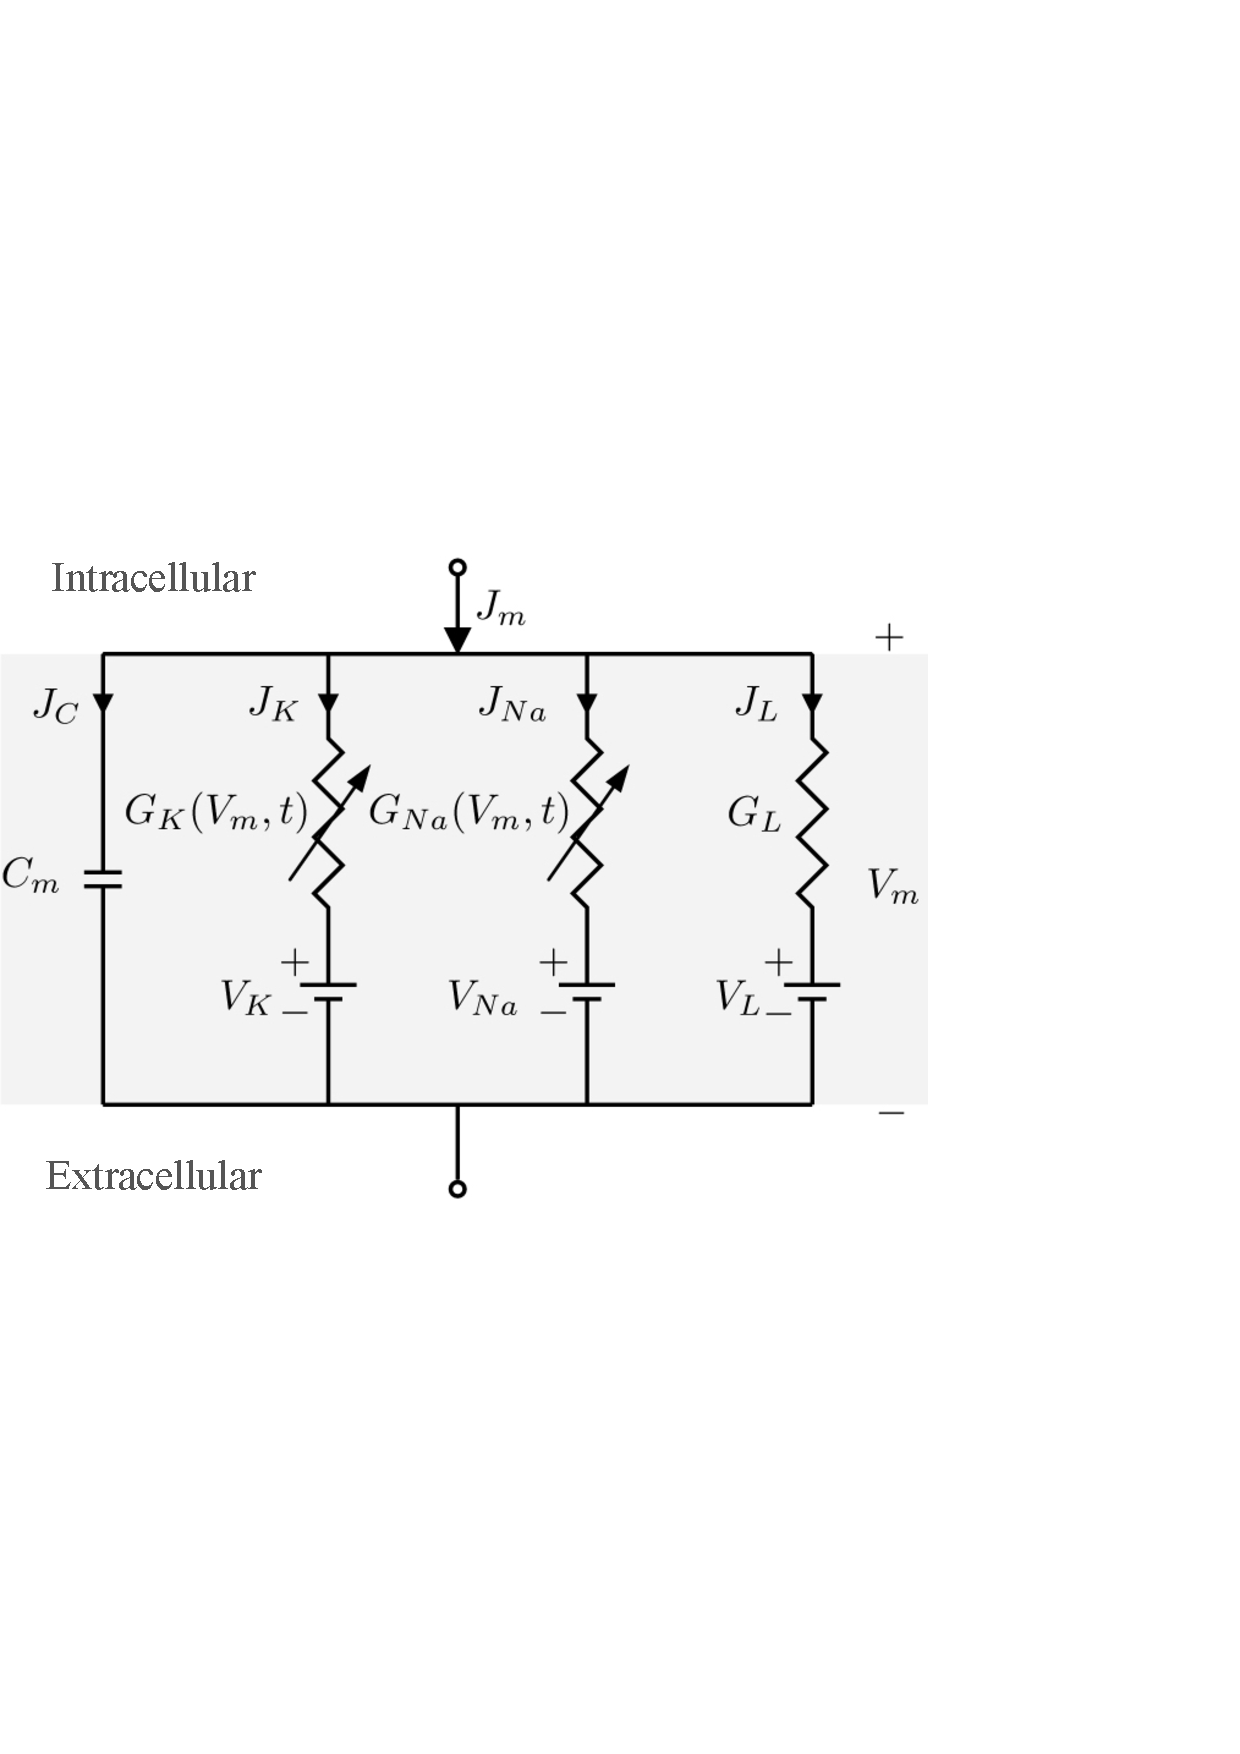
\includegraphics[width=.3\columnwidth]{AP_Conductance_Model}
\end{minipage}

\begin{minipage}{.25\columnwidth}
    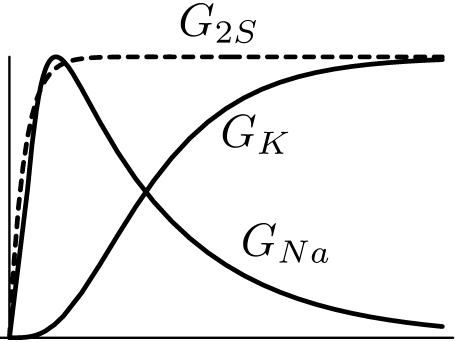
\includegraphics[width=.8\columnwidth]{AP_Conductance}
\end{minipage}
\begin{minipage}{.75\columnwidth}
    \begin{itemize}
        \item slow onset; decays slow
        \item \ce{K+} inactivates \ce{Na+} channels
    \end{itemize}
    $\to$ \textbf{Refractoriness} {\scriptsize(kurzzeitige AP Resistenz)}\\
    \phantom{$\to$} (\ce{Na+} channels are still inactivate, $h\sim0$)
\end{minipage}
%%%%%%%%%%%%%%%%%%%%%%%%%%%%%%%%%%%%%%%%%%%%%%%%%%%%%%
\subsection{Multiple states gate}
%
\formtex{open $n_Q(V_m,t)$}{big/small $Q$ $\to$ fast/slow dynamics}

\formtex{Let's write}{%
    \fbox{$h$} $= n_{-Q}$ ``slow''\!, \;\;
    \fbox{$m$} $= n_{2Q}$ ``fast''\!, \;\;
    \fbox{$n$} $= n_Q$ %``normal''
}
\formtex{~}{The \textit{lower} $T$, the \textit{bigger} the diff. between them.}
%%%%%%%%%%%%%%%%%%%%%%%%%%%%%%%%%%%%%%%%%%%%%%%%%%%%%%
\subsection{Hodkin-Huxley \textnormal{(HH)} model}
%
Experimentally you may fit the \ce{K+} and \ce{Na+} current into
\formula{Conductance}{G\ped{K}(V_m,t) = \overline{G}\ped{K} \; n^4}
\formula{~}{{G\ped{Na}(V_m,t) = \overline{G}\ped{Na} \; m^3 h}}

\begin{minipage}{.35\columnwidth}
    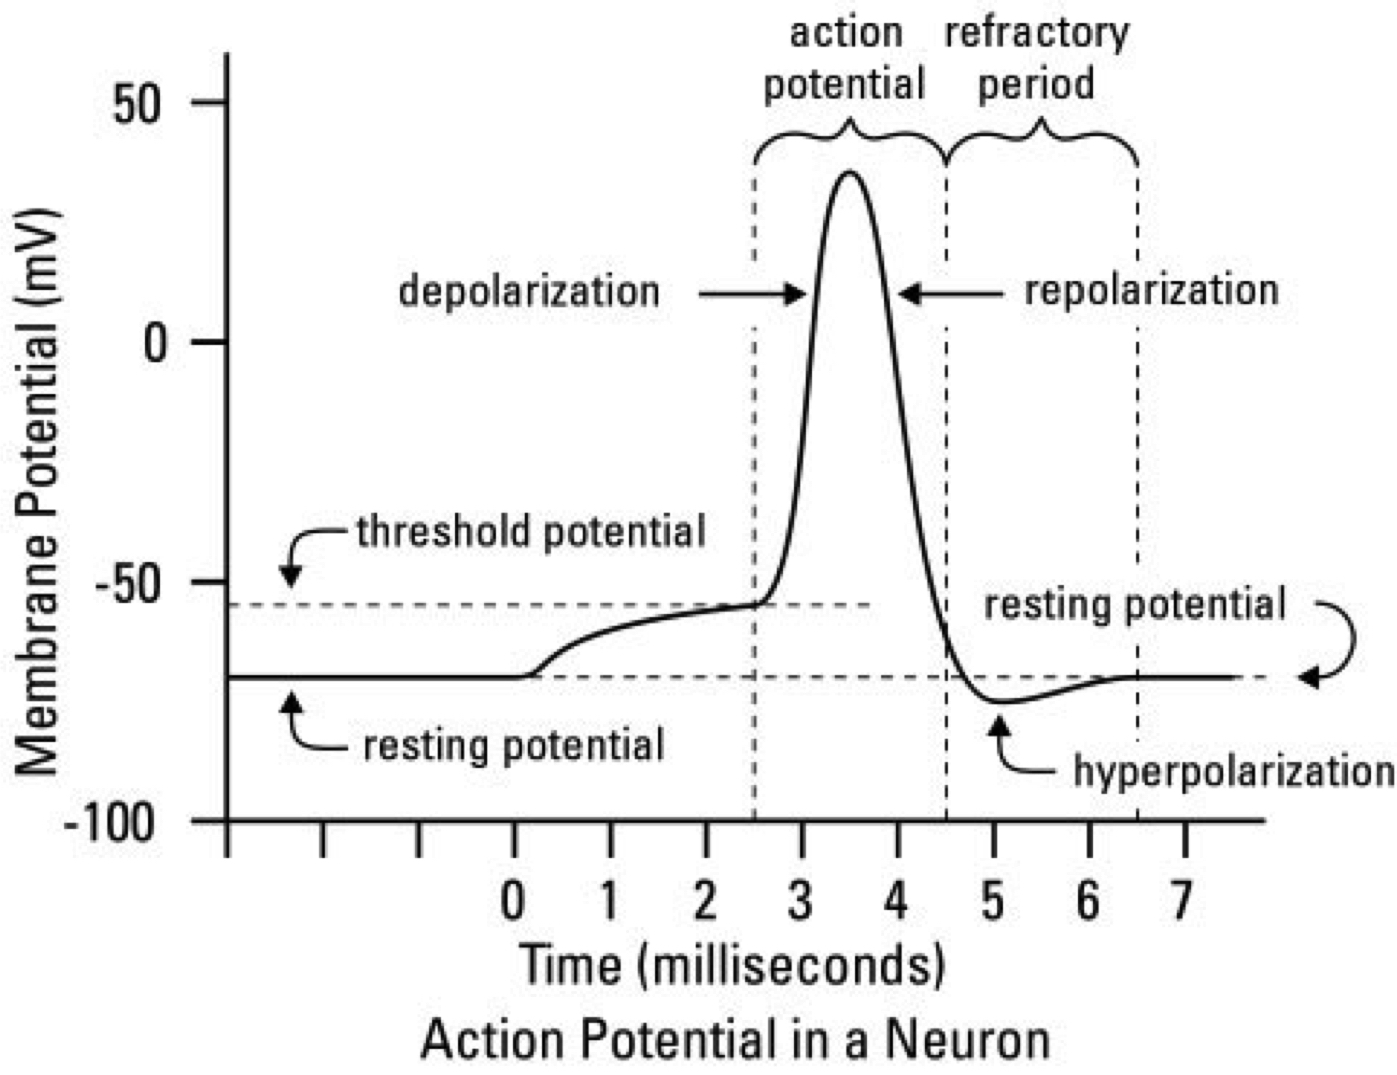
\includegraphics[width=.9\columnwidth]{AP_Actionpotential}
\end{minipage}%
\hspace{\boxmargin}%
\begin{minipage}{.65\columnwidth}
    \textbf{Four regimes during AP}:
    \begin{enumerate}
        \item[II] \textit{De}polarization:
        \ce{Na+} gate opens $\to$ \ce{Na+} in
        \item[III] \textit{Re}polarization:
        \ce{K+} gate opens $\to$ \ce{K+} out
        \item[IV] \textit{Hyper}polarization:\\
        Active \ce{Na+-K+-ion} pump (\ce{Na+}$\leftrightarrow$ \ce{K+})
    \end{enumerate}
\end{minipage}%
%%%%%%%%%%%%%%%%%%%%%%%%%%%%%%%%%%%%%%%%%%%%%%%%%%%%%%
\subsection{Decrement-free conduction}
%%%%%%%%%%%%%%%%%%%%%%%%%%%%%%%%%%%%%%%%%%%%%%%%%%%%%%
\subsubsection{Core -- Conductor Model}
%
\begin{minipage}{.3\columnwidth}
    \vspace{6mm}$V_m \big\downarrow$
    \begin{minipage}{.5\columnwidth}
        \vspace{-6mm}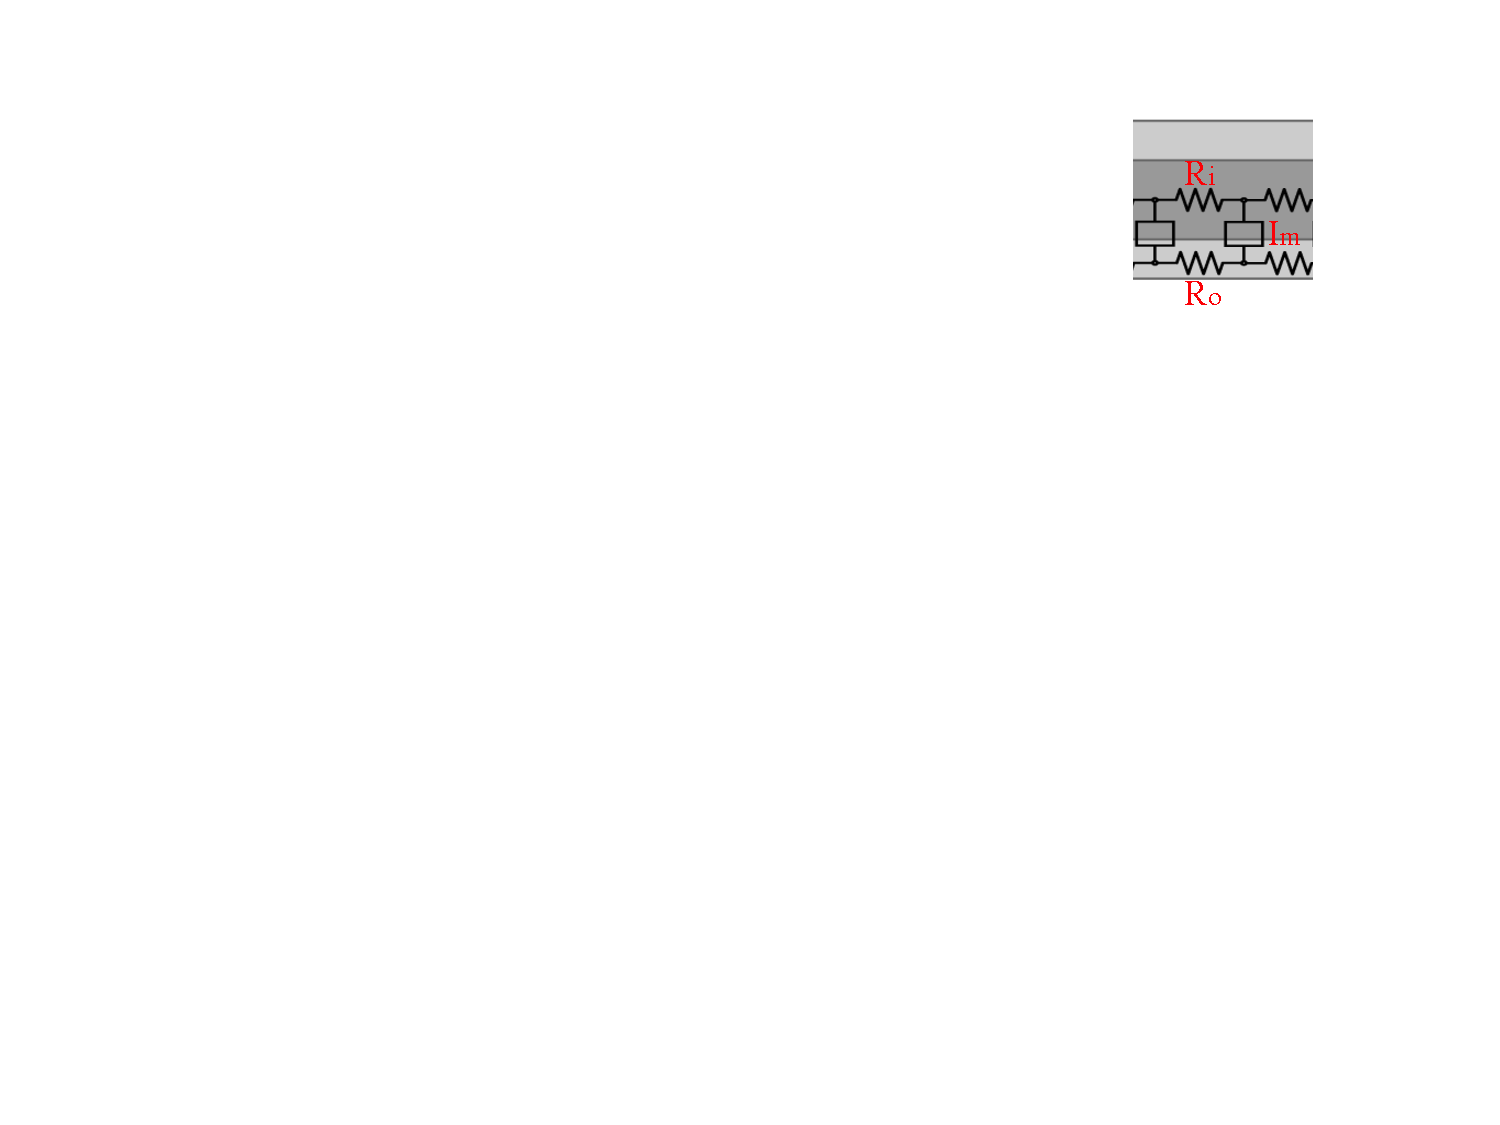
\includegraphics[width=\columnwidth]{AP_Core_Conductor_Model}
    \end{minipage}
\end{minipage}%
\hspace{1.5\boxmargin}%
\begin{minipage}{.6\columnwidth}
    $R_i = r_i \diff z$\quad $\leftarrow$ $\diff z$: per unit length\\
    $R_o = r_o \diff z$\\
    $I_m = k_m \diff z$\quad $\leftarrow$ may use HH-model
\end{minipage}%

\vspace{-3mm}
\formula{Core--Conductor eq.}{\pderiv[2]{V_m(z,t)}{z} = (r_o+r_i)K_m(z,t) - \overbrace{r_oK_e(z,t)}^{\overset{\textrm{if}}{=}\; 0 \;\to\; I_o = -I_i}}
\formula{\hfill wave eq.}{\phantom{\pderiv[2]{V_m(z,t)}{z}} = \frac{1}{v^2} \pderiv[2]{V_m(z,t)}{t} }
\enskip with $v = \frac{W}{\Delta t}$
\formbox{\hfill$\overset{K_e=0}{\implies}$}{v \simeq \frac{K_ma}{2\rho_i}}
\enskip for $r_i \gg r_o$
\enskip i.e. $v\propto\sqrt{a}$
%%%%%%%%%%%%%%%%%%%%%%%%%%%%%%%%%%%%%%%%%%%%%%%%%%%%%%
\subsubsection{Cable model \textnormal{-- Core--Conductor with HH-model inside}}
%
\formtex{Linearize \small(1st order)}{\small timescale for membrane voltage changes {$\tau_m {=} \frac{C_m}{G_m}$}}
\formtex{Cable equation}{Let $v_m = V_m + V_m\ap{rest}$}
~\qquad $v_m {+} \hspace{-1mm}\underbrace{\tau_m\pderiv{v_m}{t}\vspace{-1mm}}_{\vspace{-2mm} = 0 \text{ time indep.}}\hspace{-1mm} - \lambda_C^2 \pderiv[2]{v_m}{z} {=} r_o\lambda_C^2K_e$
\enskip \highlight{$\lambda_C {=} \frac{1}{\sqrt{g_m(r_o+r_i)}}$}
%%%%%%%%%%%%%%%%%%%%%%%%%%%%%%%%%%%%%%%%%%%%%%%%%%%%%%
\subsubsection{Saltatory Conduction Hypothesis}
%
$\to$ explain discrete manner in steps

\formula{velocity $\sim$ axon}{\textrm{total delay} \sim N (\#\textrm{nodes}) \sim (\textrm{axon length})/L}
\formula{diameter $D$}{\ce{->[$L\sim D$]} \textrm{velocity} \sim \frac{\textrm{total delay}}{\textrm{axon length}} \sim D}

\begin{minipage}{\columnwidth/3}
    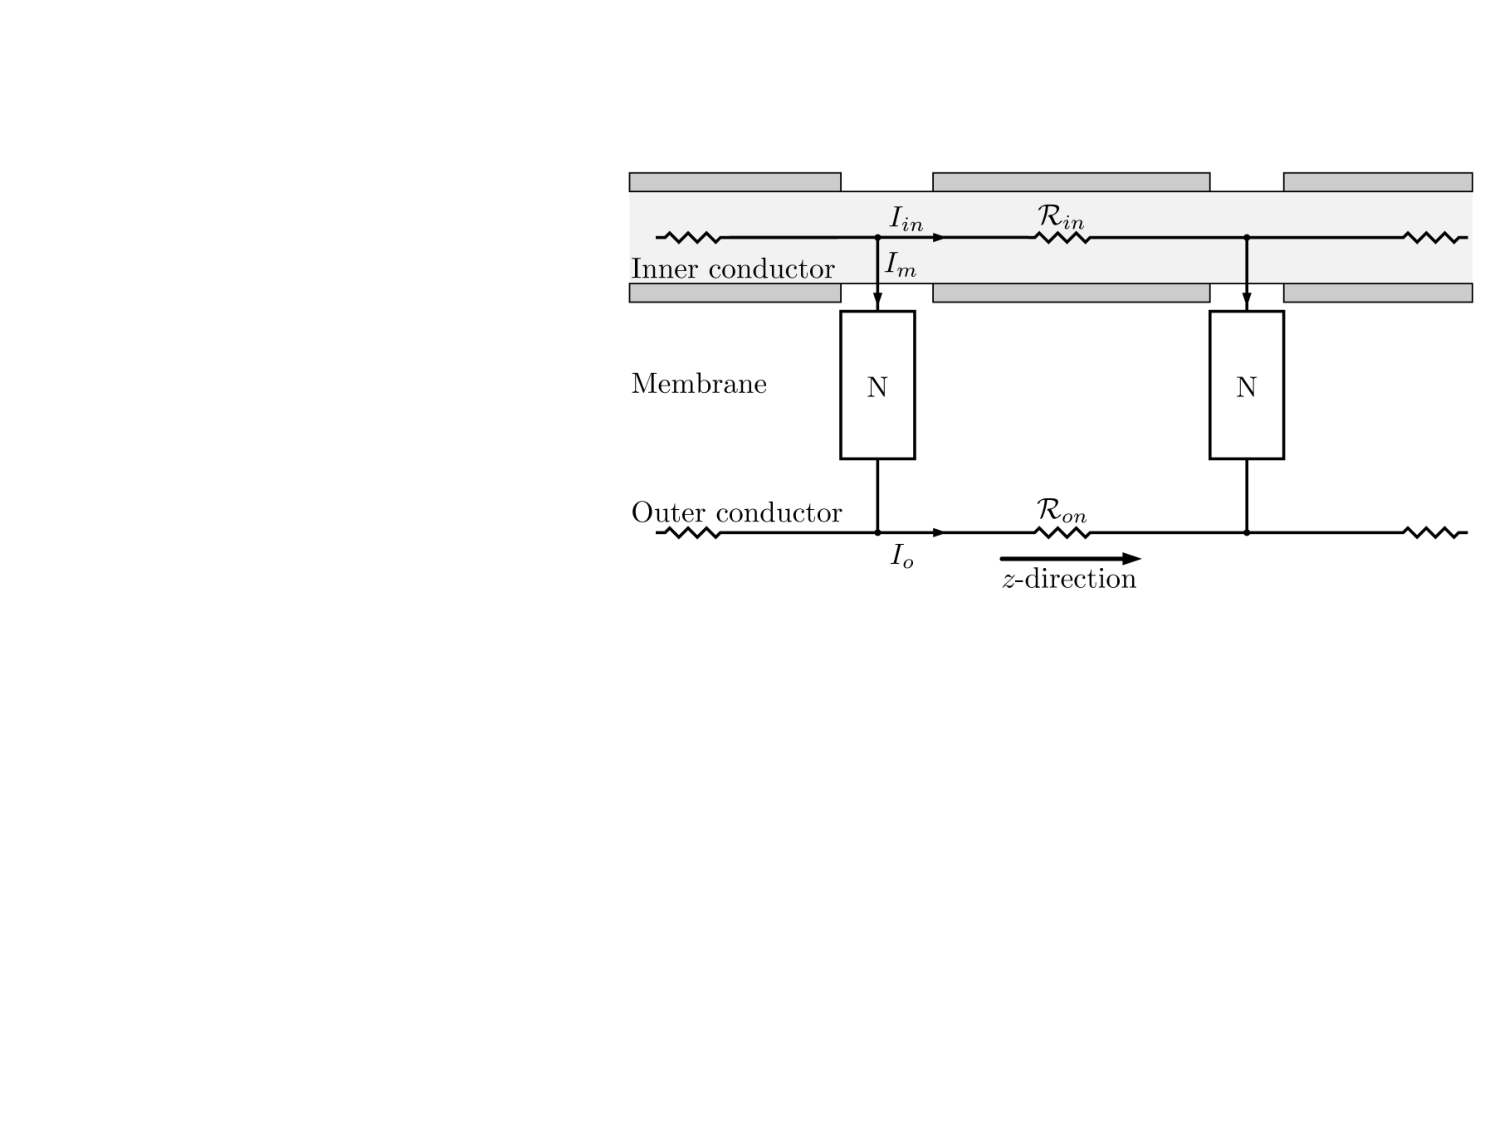
\includegraphics[width=.85\columnwidth]{AP_Saltatory}
\end{minipage}%
\begin{minipage}{\columnwidth/3}
    \centering
    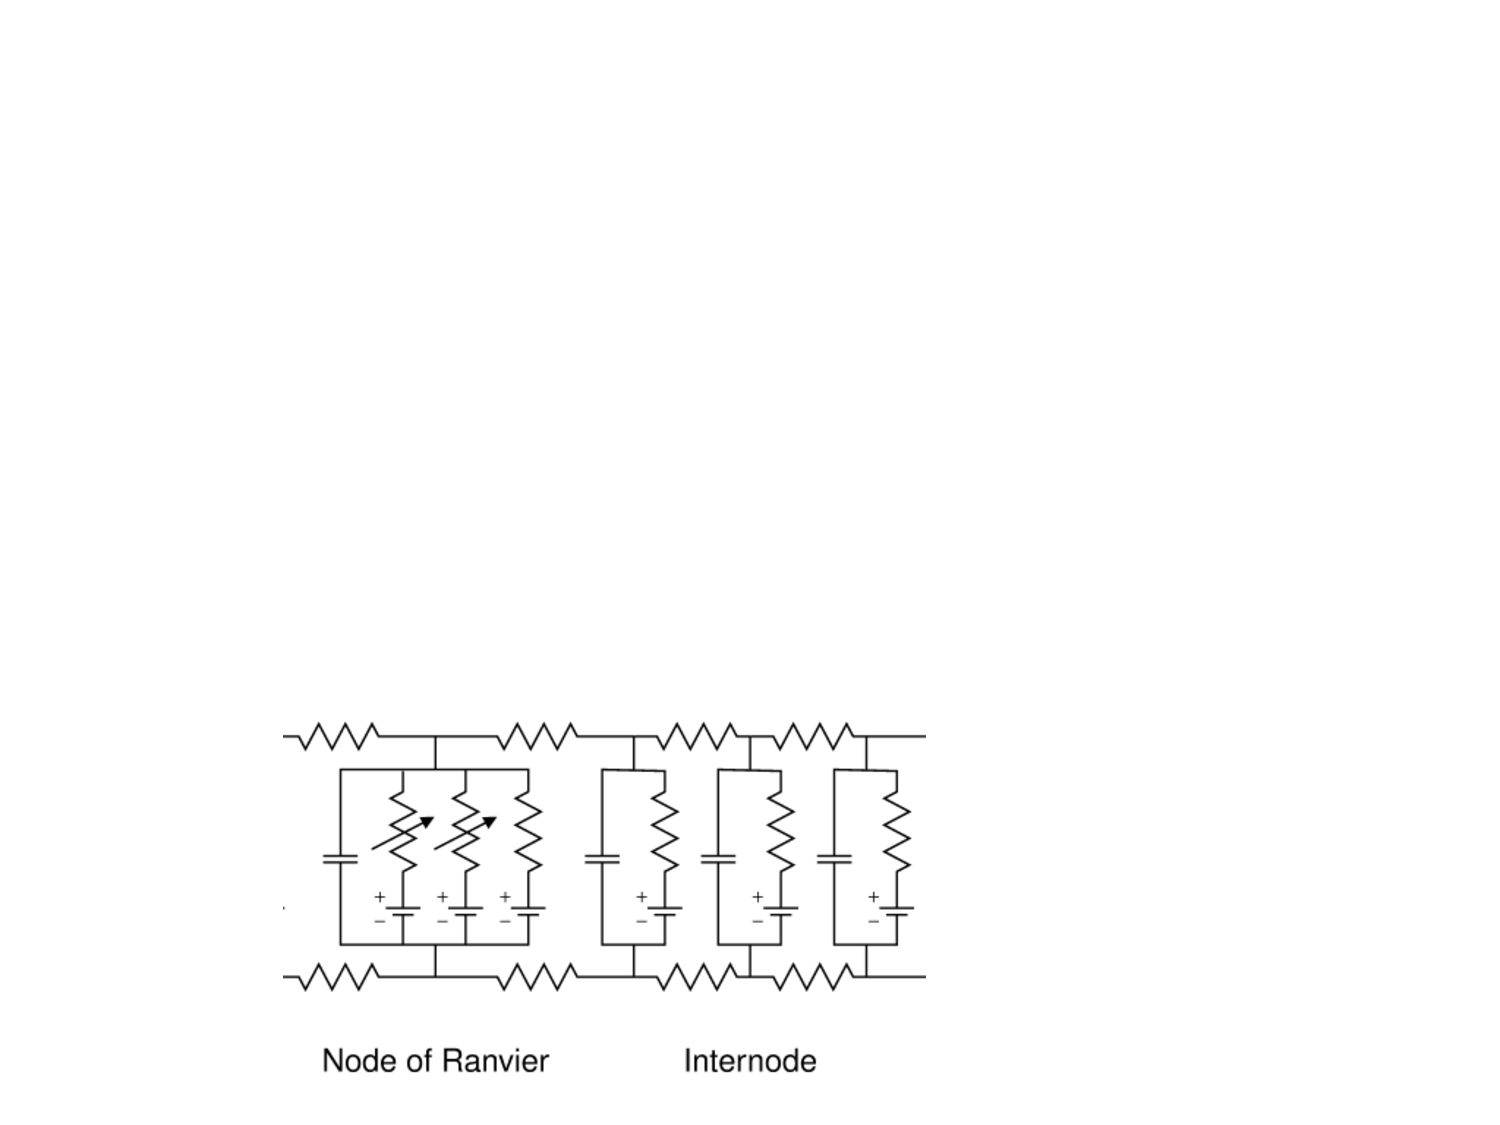
\includegraphics[width=.8\columnwidth]{AP_Saltatory_2}
\end{minipage}%
\begin{minipage}{\columnwidth/3}
    \hfill
    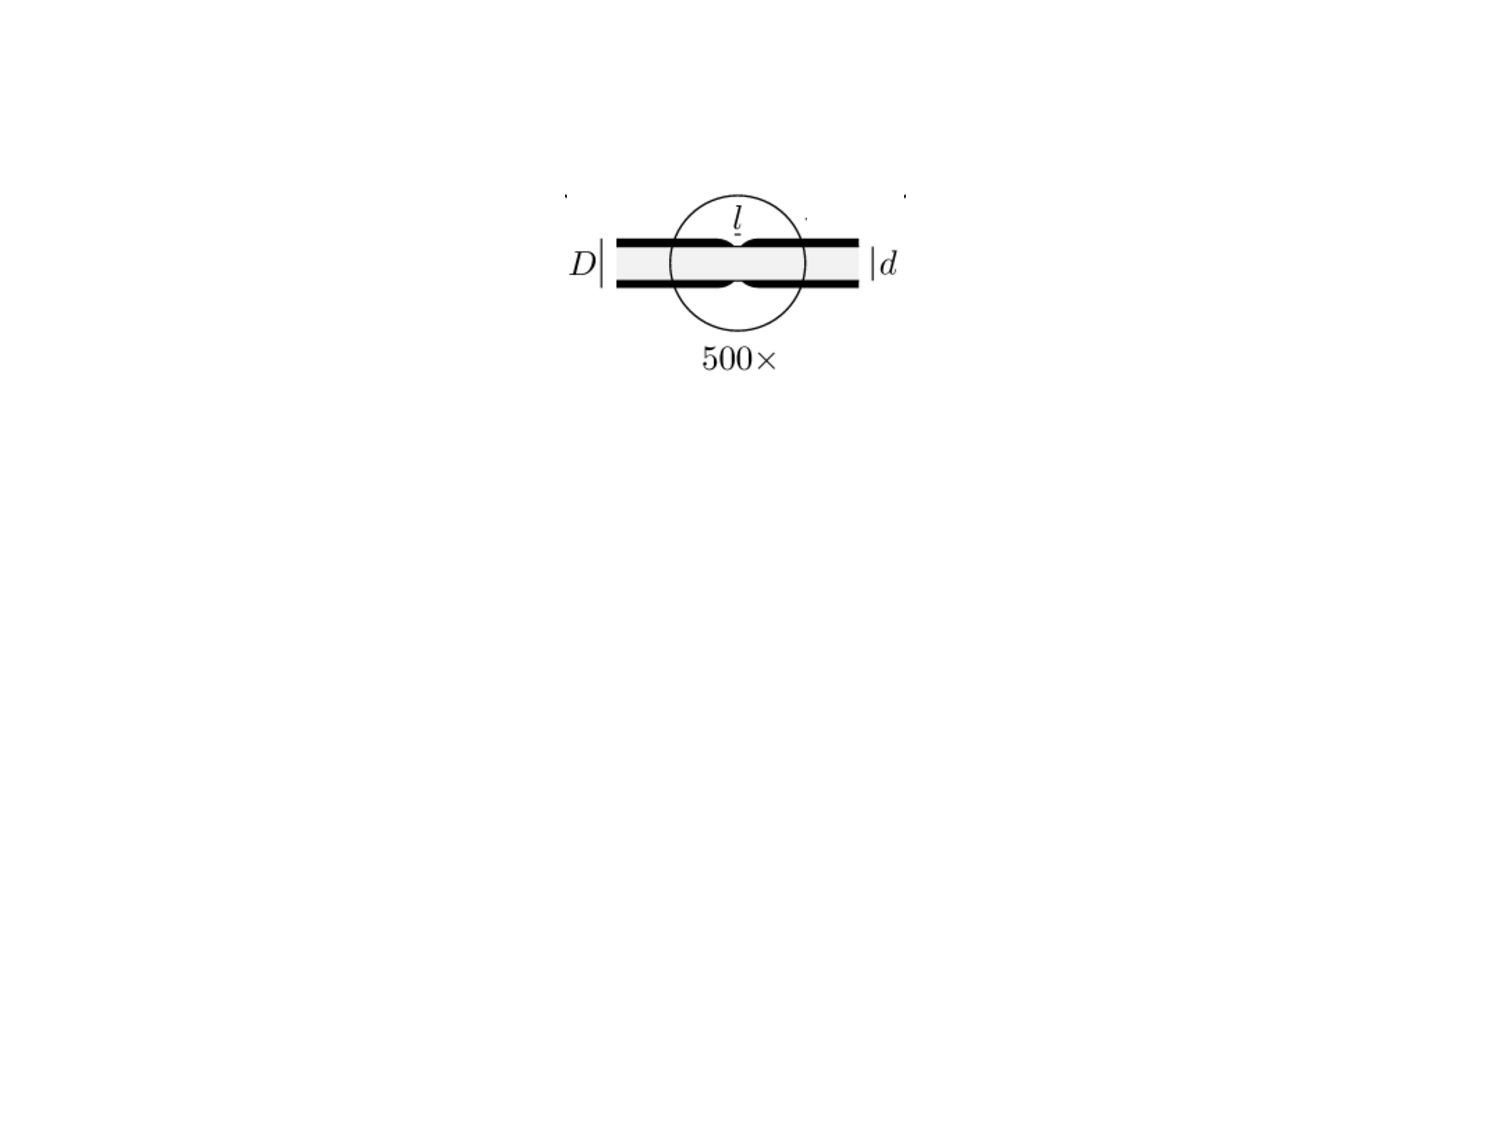
\includegraphics[width=.75\columnwidth]{AP_Ranvier_Node}
\end{minipage}
